\setminted{texcomments=off}

%------------------------------------------------------------------------------
\section{Doing Stuff With Contracts}
%------------------------------------------------------------------------------
\begin{frame}
  \tableofcontents[currentsection,hidesubsections]
\end{frame}


\subsection{A Dream}
%------------------------------------------------------------------------------
\begin{frame}
  \note{6 Minutes}

  \frametitle{Proven contracts}

  \begin{itemize}
  \item Prove software correctness \pause
    \item Encode contracts completely \pause
      \begin{itemize}
      \item All preconditions \pause
      \item All postconditions \pause
      \item All essential behavior \pause
      \end{itemize}
    \item Statically prove everything \pause
      \begin{itemize}
      \item For each function, prove postconditions and essential behavior \pause
      \item Use called functions contracst in proofs of larger functions \pause
      \end{itemize}
    \item PROFIT
  \end{itemize}
  
  % see p1773/p1774 for motivation?

%  \begin{cppcodebox}
%    int get_size() [[ post r : r >= 0 ]];
%    
%    int div32(int x) [[ pre : x >= 0 ]]
%    { return x / 32; }
%
%    int foo(int x)
%    {
%        return div32(get_size());
%    }   
%  \end{cppcodebox}
\end{frame}

\begin{frame}
  \frametitle{Dream Benefit \#1 - Less Bugs}
  \pause
  \begin{itemize}
  \item Compiler identifies all violated contracts \pause
  \item Edge cases must be throught through \pause
  \item All assumptions are captured in compiled code \pause
  \item Mostly, if it compiles, it doesn't have bugs (contract violations) \pause
  \item If there is a bug, contracts just need to be elaborated
  \end{itemize}
\end{frame}

\begin{frame}
  \frametitle{Dream Benefit \#2 - Less Heat Generation}
  \pause
  \begin{itemize}
  \item No need for any checks \pause
  \item More knowledge for the compiler \pause
    \begin{itemize}
    \item \cc{__builtin_assume} \pause
    \item Removing excess branches \pause
    \item Vectorization/SIMD instructions \pause
    \end{itemize}
  \item Smaller code size
  \end{itemize}
\end{frame}

\begin{frame}
  \frametitle{Realizing parts of the dream}
  \begin{itemize}
  \item WARNING: \pause MACROS INCOMING \pause
    
  \item How to leverage contracts without a language feature \pause
  \item Bloomberg has been doing this for 15 years \pause
  \item See the BDE open source repostory for the real implementation
    \begin{itemize}
      \item \adjustbox{width=0.8\textwidth}{\url{https://github.com/bloomberg/bde/blob/master/groups/bsl/bsls/bsls_assert.h}}
      \item \adjustbox{width=0.8\textwidth}{\small \url{https://github.com/bloomberg/bde/blob/master/groups/bsl/bsls/bsls_review.h}}
    \end{itemize}
  \end{itemize}
\end{frame}

\subsection{Less Bugs}
%------------------------------------------------------------------------------
\begin{frame}
  What do you do if you can't prove a contract is being followed? \\
  \\ \pause
  \center{\Huge{Experiment}}
\end{frame}
  

\begin{frame}
  \tableofcontents[currentsection,currentsubsection,subsectionstyle=show/shaded/hide]
\end{frame}

\begin{frame}[fragile]
  \note{10 Minutes}
  
  \frametitle{Documenting expectations}

  \begin{itemize}
  \item<1-> Initial benefit of contracts in code 
  \item<3-> Bloomberg specific naming
  \item<4-> Avoid code rot
  \item<5-> ... wish we had done that originally
  \item<6-> ... or at least this to require a \cc{;}
  \item<7-> For simplicity
  \end{itemize}
\begin{overprint}
\onslide<2,7>
\begin{cppcodebox}
#define ASSERT(X)
\end{cppcodebox}

\onslide<3>
\begin{cppcodebox}
#define BSLS_ASSERT(X)
\end{cppcodebox}

\onslide<4>
\begin{cppcodebox}
#define BSLS_ASSERT(X) sizeof( (X)?true:false )    
\end{cppcodebox}

\onslide<5>
\begin{cppcodebox}
#ifdef BSLS_ASSERT_VALIDATE_DISABLED_MACROS
#define BSLS_ASSERT(X) sizeof( (X)?true:false )
#else
#define BSLS_ASSERT(X)
#endif
\end{cppcodebox}

\onslide<6>
\begin{cppcodebox}
#define BSLS_ASSERT(X) ((void)0)
\end{cppcodebox}

\end{overprint}

\end{frame}

\begin{frame}[fragile]
  \frametitle{Aborting on bugs}

  \begin{itemize}
  \item<1-> Identifying violations would be nice
  \item<2-> The safest thing to do is stop immediately
  \item<3-> Nice if \cc{ASSERT(X)} needs a semicolon
  \item<4-> For simplicity
  \end{itemize}
\begin{overprint}
\onslide<2,4>
\begin{cppcodebox}
#define ASSERT(X) if (!(X)) { std::abort(); }
\end{cppcodebox}

\onslide<3>
\begin{cppcodebox}
#define ASSERT(X) do { if (!(X)) { std::abort(); } } while (false)
\end{cppcodebox}

\end{overprint}

\end{frame}

\begin{frame}[fragile]
  \frametitle{... only in some builds}

  \begin{itemize}
  \item<1-> Checks of contracts are redundant if they're not broken
  \item<2-> NDEBUG might be a way to control enablement
  \item<3-> This reminds me of something
  \item<4-> Separating out controls from behavior helps
  \end{itemize}

\begin{overprint}
\onslide<2>
\begin{cppcodebox}
#ifdef NDEBUG
#define ASSERT(X)
#else
#define ASSERT(X) if (!(X)) { std::abort(); }
#endif
\end{cppcodebox}

\onslide<3>
\begin{cppcodebox}
#include <cassert>
#define ASSERT(X) assert(X)
\end{cppcodebox}

\onslide<4>
\begin{cppcodebox}
#define ASSERT_IMP(X)          if (!(X)) { std::abort(); }
\end{cppcodebox}

\onslide<5>
\begin{cppcodebox}
#define ASSERT_IMP(X)          if (!(X)) { std::abort(); }
#define ASSERT_DISABLED_IMP(X)
\end{cppcodebox}

\onslide<6>
\begin{cppcodebox}
#define ASSERT_IMP(X)          if (!(X)) { std::abort(); }
#define ASSERT_DISABLED_IMP(X)

#ifdef ASSERT_LEVEL_ASSERT
#define ASSERT(X) ASSERT_IMP(X)
#else
#define ASSERT(X) ASSERT_DISABLED_IMP(X)
#endif
\end{cppcodebox}

\end{overprint}
  
\end{frame}

\begin{frame}<1-3>[fragile,label=whathappened]
  \frametitle{... but what happened?}
\begin{itemize}
\item<1-> Aborting with no information sucks
\item<2-> Logging something helps
\item<3-> The preprocessor can give us more help
\item<4-> Delegating to a pluggable function helps that
\item<6-> Leave all behavior up to the violation handler
\end{itemize}
\begin{overprint}
\onslide<1>
\begin{cppcodebox}
#define ASSERT_IMP(X) if (!(X)) {                                   \
    /*POOF*/;                                                       \
    std::abort();                                                   \
}
\end{cppcodebox}

\onslide<2>
\begin{cppcodebox}
#define ASSERT_IMP(X) if (!(X)) {                                   \
    printf("ASSERTION FAILED!\n");                                  \
                                                                    \
    std::abort();                                                   \
}
\end{cppcodebox}

\onslide<3>
\begin{cppcodebox}
#define ASSERT_IMP(X) if (!(X)) {                                   \
    printf("ASSERTION FAILED (" __FILE__ ":%d): %s\n",              \
                                __LINE__, #X);                      \
    std::abort();                                                   \
}
\end{cppcodebox}

\onslide<4>
\begin{cppcodebox}
#define ASSERT_IMP(X) if (!(X)) {                                   \
    bb::Assert::invoke_violation_handler(__FILE__, __LINE__, #X);   \
                                                                    \
    std::abort();                                                   \
}
\end{cppcodebox}

\onslide<5>
\begin{cppcodebox}
#define ASSERT_IMP(X) if (!(X)) {                                   \
    bb::assert_violation violation(__FILE__, __LINE__, #X); \
    bb:Assert::invoke_violation_handler(violation);                 \
    std::abort();                                                   \
}
\end{cppcodebox}

\onslide<6>
\begin{cppcodebox}
#define ASSERT_IMP(X) if (!(X)) {                                   \
    bb::assert_violation violation(__FILE__, __LINE__, #X);         \
    bb::Assert::invoke_violation_handler(violation);                \
}
\end{cppcodebox}

\onslide<7>
\begin{cppcodebox}
void bb::Assert::invoke_violation_handler(
                            const bb::assert_violation &violation) {
    getViolationHandler()(violation);
}
\end{cppcodebox}

\onslide<8>
\begin{cppcodebox}
void xkcd::violationHandler(const bb::assert_violation &violation) {
  printf("Error\n");
  printf("If you're seeing this, the code is in what\n");
  printf("I thought was an unreachable state.");
  //...
}
\end{cppcodebox}

\onslide<9>
\begin{cppcodebox}
  int main() {
    bb::Assert::setViolationHandler(&xkcd::violationHandler);
    //..
  }
\end{cppcodebox}

\end{overprint}
\end{frame}

\begin{frame}
  \frametitle{What about this guy?}
  \begin{figure}
    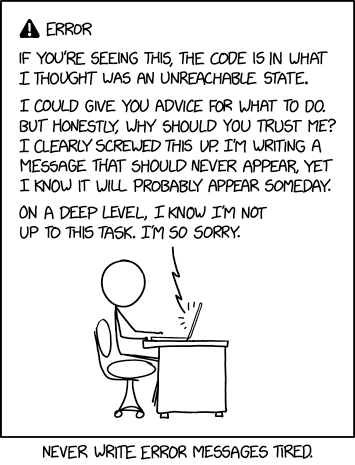
\includegraphics[height=0.9\textheight]{xkcdunreachablestate}
    \caption{https://xkcd.com/2200/}
  \end{figure}
\end{frame}

\againframe<4->{whathappened}

\begin{frame}[fragile]
  \frametitle{... that doesn't work everywhere!}

  \begin{itemize}
  \item The violation handler can notify in different ways \pause
    \begin{itemize}
    \item Custom logging frameworks \pause
    \item GUI messages (abort, retry, fail?) \pause
    \item Hardware notifications \pause
    \end{itemize}
  \item ... do different things \pause
    \begin{itemize}
    \item \cc{std::abort()} \pause
    \item \cc{while (true) {std::this_thread::sleep_for(std::chrono::years(1));}} \pause
    \item \cc{throw std:::exception("Oops?");} \pause
    \end{itemize}
  \item ... or try to recover? \pause
  \item \cc{main} gets to decide
  \end{itemize}
\end{frame}

\begin{frame}[fragile]
  \frametitle{Checking is slow!}

  \begin{itemize}
  \item<1-> Checks use state already in cache, are often very fast 
  \item<2-> Algorithmic complexity can still ruin that 
  \item<3-> 3 levels of complexity 
  \item<4-> ... 2 levels probably sufficient 
  \item<5-> Linear scale of enablement
  \item<13-> Bloomberg 2005-2018
  \end{itemize}

\begin{overprint}
\onslide<1>
\begin{cppcodebox}
T* binsearch(T*begin, T*end, const T& val) {
  ASSERT(begin);
  ASSERT(end);
  ASSERT(begin < end)7
  //..
}
\end{cppcodebox}

\onslide<2>
\begin{cppcodebox}
T* binsearch(T*begin, T*end, const T& val) {
  ASSERT(is_sorted_range(begin,end));
  //..
}
\end{cppcodebox}

\onslide<3>
\begin{cppcodebox}
#define ASSERT_OPT(X) ...
#define ASSERT(X) ...
#define ASSERT_SAFE(X) ...
\end{cppcodebox}

\onslide<4>
\begin{cppcodebox}
[[ assert default : X ]];
[[ assert audit : X ]];
\end{cppcodebox}

\onslide<5>
\begin{cppcodebox}
#if defined(ASSERT_LEVEL_NONE)   ? 1 : 0 \
  + defined(ASSERT_LEVEL_OPT)    ? 1 : 0 \
  + defined(ASSERT_LEVEL_ASSERT) ? 1 : 0 \
  + defined(ASSERT_LEVEL_SAFE)   ? 1 : 0 \
  > 1
#error Multiple ASSERT_LEVEL macros defined
#endif
\end{cppcodebox}

\onslide<6>
\begin{cppcodebox}
#if !defined(ASSERT_LEVEL_NONE)   \
 && !defined(ASSERT_LEVEL_OPT)    \
 && !defined(ASSERT_LEVEL_ASSERT) \
 && !defined(ASSERT_LEVEL_SAFE)
#define ASSERT_LEVEL_ASSERT
#endif
\end{cppcodebox}

\onslide<7>
\begin{cppcodebox}
#if defined(ASSERT_LEVEL_NONE)
#define ASSERT_OPT(X)  ASSERT_DISABLED_IMP(X)
#define ASSERT(X)      ASSERT_DISABLED_IMP(X)
#define ASSERT_SAFE(X) ASSERT_DISABLED_IMP(X)
//..  
\end{cppcodebox}

\onslide<8>
\begin{cppcodebox}
//..
#elif defined(ASSERT_LEVEL_OPT)
#define ASSERT_OPT(X)  ASSERT_IMP(X)
#define ASSERT(X)      ASSERT_DISABLED_IMP(X)
#define ASSERT_SAFE(X) ASSERT_DISABLED_IMP(X)
//..  
\end{cppcodebox}

\onslide<9>
\begin{cppcodebox}
//..
#elif defined(ASSERT_LEVEL_ASSERT)
#define ASSERT_OPT(X)  ASSERT_IMP(X)
#define ASSERT(X)      ASSERT_IMP(X)
#define ASSERT_SAFE(X) ASSERT_DISABLED_IMP(X)
//..  
\end{cppcodebox}

\onslide<10>
\begin{cppcodebox}
//..
#elif defined(ASSERT_LEVEL_SAFE)
#define ASSERT_OPT(X)  ASSERT_IMP(X)
#define ASSERT(X)      ASSERT_IMP(X)
#define ASSERT_SAFE(X) ASSERT_IMP(X)
#endif
\end{cppcodebox}

\onslide<11>
\begin{cppcodebox*}{highlightlines={4,7}}
#if defined(ASSERT_LEVEL_OPT)    \
 || defined(ASSERT_LEVEL_ASSERT) \
 || defined(ASSERT_LEVEL_SAFE)
#define ASSERT_OPT(X) ASSERT_IMP(X)
#else
 // defined(ASSERT_LEVEL_NONE)
#define ASSERT_OPT(X) ASSERT_DISABLED_IMP(X)
#endif
\end{cppcodebox*}

\onslide<12>
\begin{cppcodebox*}{highlightlines={3,7}}
#if defined(ASSERT_LEVEL_ASSERT) \
 || defined(ASSERT_LEVEL_SAFE)
#define ASSERT(X) ASSERT_IMP(X)
#else
 // defined(ASSERT_LEVEL_OPT)
 // defined(ASSERT_LEVEL_NONE)
#define ASSERT(X) ASSERT_DISABLED_IMP(X)
#endif
\end{cppcodebox*}

\onslide<13>
\begin{cppcodebox*}{highlightlines={2,7}}
#if defined(ASSERT_LEVEL_SAFE)
#define ASSERT_SAFE(X) ASSERT_IMP(X)
#else
 // defined(ASSERT_LEVEL_OPT)
 // defined(ASSERT_LEVEL_ASSERT)
 // defined(ASSERT_LEVEL_NONE)
#define ASSERT_SAFE(X) ASSERT_DISABLED_IMP(X)
#endif
\end{cppcodebox*}

\end{overprint}
\end{frame}


\subsection{Deploying it}
%------------------------------------------------------------------------------
\begin{frame}
  \tableofcontents[currentsection,currentsubsection,subsectionstyle=show/shaded/hide]
\end{frame}

\begin{frame}
  \frametitle{Choosing Levels in code}
  \begin{itemize}
  \item Original Suggestion:\pause
    \begin{itemize}
    \item \cc{OPT}: 5\% most critical tests \pause
    \item \cc{ASSERT}: 90\% tests <2x performance hit \pause
    \item \cc{SAFE}: 5\% anything slower \pause
    \end{itemize}
  \item Current Suggestion:\pause
    \begin{itemize}
    \item \cc{OPT}: 0-0.5\% absolutely critical and 0-impact \pause
    \item \cc{ASSERT}: 99\% non $O(n)$-impacting \pause
    \item \cc{SAFE}: 0.5-1\% algorithmicly slow \pause
    \end{itemize}
  \item Changing is hard
  \end{itemize}

\end{frame}
  
\begin{frame}
  \frametitle{Choosing Levels in builds}
  \begin{itemize}
  \item What we did \pause
    \begin{itemize}
    \item Developement - \cc{ASSERT_LEVEL_ASSERT} \pause
    \item Unit tests - \cc{ASSERT_LEVEL_ASSERT} hopefully \pause
    \item Beta testing - \cc{ASSERT_LEVEL_ASSERT_OPT} \pause
    \item Production - \cc{ASSERT_LEVEL_ASSERT_OPT} \pause
    \end{itemize}
  \item What we wanted \pause
    \begin{itemize}
    \item Developement - \cc{ASSERT_LEVEL_ASSERT} or \cc{ASSERT_LEVEL_SAFE} \pause
    \item Unit tests - \cc{ASSERT_LEVEL_ASSERT} or \cc{ASSERT_LEVEL_SAFE} \pause
    \item Beta testing - \cc{ASSERT_LEVEL_ASSERT} or \cc{ASSERT_LEVEL_SAFE} \pause
    \item Production - \cc{ASSERT_LEVEL_ASSERT} \pause
    \end{itemize}
  \item ... which is where we are 
  \end{itemize}
\end{frame}

\begin{frame}
  \frametitle{The Next Step}

  \begin{itemize}
  \item Adding more assertions \pause
    \begin{itemize}
    \item \cc{~bsl::string() { ASSERT(m_data[m_size] == 0); }} \pause
    \item Time ABI change \pause
    \end{itemize}
  \item Changing levels of assertions \pause
    \begin{itemize}
    \item SAFE to ASSERT \pause
    \item ASSERT to OPT \pause
    \end{itemize}
  \item Changing deployed assertion levels \pause
  \item Everyone will need to do this in 202x! \pause
    \begin{itemize}
    \item Using language contracts when they come will be a case of adding new assertions to existing code.
    \end{itemize}
  \end{itemize}
\end{frame}

\begin{frame}
  \frametitle{Mis-Step \#1}

  \begin{itemize}
  \item Continuing violation handler (2008-2015) \pause
    \begin{itemize}
    \item Requires cooperation from main \pause
    \item Allows new bugs to go through unnoticed \pause
    \item At least 1 major Bloomberg (WP) bug was because of this \pause
    \item Blanket continuation unsafe
    \end{itemize}
  \end{itemize}
\end{frame}

\begin{frame}
  \frametitle{Mis-Step \#2}
  \begin{itemize}
  \item Extra Smart violation handler (~2016) \pause
    \begin{itemize}
    \item Configuration to allow continuation \pause
    \item Tracking failure counts \pause
    \item Alternate logging \pause
    \end{itemize}
  \item Still unsuccessful \pause
    \begin{itemize}
    \item Requires even more cooperation from main \pause
    \item No way to indicate in code that a check is ``new'' \pause
    \item Rarely used, minimal progress
    \end{itemize}
  \end{itemize}
\end{frame}

\begin{frame}
  \frametitle{Step?}

  \begin{itemize}
  \item \cc{BSLS_REVIEW} (2018) \pause
    \begin{itemize}
    \item No explicit cooperation from main needed \pause
    \item Contracts can be marked as ``new'' in code \pause
    \item Build-time controls to mark all assertions at a level as ``new'' \pause
    \end{itemize}
  \end{itemize}
  
\end{frame}

\begin{frame}
  \frametitle{BSLS_REVIEW overview}

  \begin{itemize}
  \item Parallel structure to \cc{BSLS_ASSERT} \pause
  \item Separate violation handler, defaults to logging \pause
  \item Lifecycle \cc{BSLS_ASSERT_SAFE} to \cc{BSLS_REVIEW} to \cc{BSLS_ASSERT} \pause
  \item Alternately, <nothing> to \cc{BSLS_REVIEW_?} to \cc{BSLS_ASSERT_?} 
  \end{itemize}

\end{frame}

\begin{frame}[fragile]
  \frametitle{BSLS_REVIEW}

  \begin{itemize}
  \item<1->Initially a copy of ASSERT
  \item<2->Number of failures is important
  \item<3->Default violation handler logs only
  \item<4->With expeonential backoff
  \end{itemize}

  \begin{overprint}
\onslide<1>
\begin{cppcodebox}
#define REVIEW_IMP(X) if (!(X)) {                                   \
    bb::assert_violation violation(__FILE__, __LINE__, #X);         \
    bb::Review::invoke_violation_handler(violation);                \
}
\end{cppcodebox}
    
\onslide<2>
\begin{cppcodebox}
#define REVIEW_IMP(X) if (!(X)) {                                   \
    static std::atomic<int> count;                                  \
    bb::review_violation violation(__FILE__, __LINE__, ++count, #X);\
    bb::Review::invoke_violation_handler(violation);                \
}
\end{cppcodebox}

\onslide<3>
\begin{cppcodebox}
void Review::default_violation_handler(
                              const bb::review_violation &violation)
{
  // Log a message, with contents of violation
  // Log a stack trace
  // Return
}
\end{cppcodebox}

\onslide<4>
\begin{cppcodebox}
void Review::default_violation_handler(
                              const bb::review_violation &violation)
{
  int count = violation.count();
  if (0 == (count & (count-1))) {
    // Log a message, with contents of violation
    // Log a stack trace
  }
  // Return
}
\end{cppcodebox}
\end{overprint}

\end{frame}

\begin{frame}[fragile]
  \frametitle{BSLS_REVIEW Build time control}

  \begin{itemize}
    \item<1-> Mutually exlusive
    \item<2-> Default to assert level \onslide<3>{(In reality copies assert logic)}
    \item<4-> Controls just like ASSERT
  \end{itemize}

\begin{overprint}
\onslide<1>
\begin{cppcodebox}
#if defined(REVIEW_LEVEL_NONE)   ? 1 : 0 \
  + defined(REVIEW_LEVEL_OPT)    ? 1 : 0 \
  + defined(REVIEW_LEVEL_REVIEW) ? 1 : 0 \
  + defined(REVIEW_LEVEL_SAFE)   ? 1 : 0 \
  > 1
#error Multiple REVIEW_LEVEL macros defined
#endif
\end{cppcodebox}

\onslide<2-3>
\begin{cppcodebox}
#if defined(ASSERT_LEVEL_NONE)
#define REVIEW_LEVEL_NONE
#elif defined(ASSERT_LEVEL_OPT)
#define REVIEW_LEVEL_OPT
#elif defined(ASSERT_LEVEL_ASSERT)
#define REVIEW_LEVEL_REVIEW
#elif defined(ASSERT_LEVEL_SAFE)
#define REVIEW_LEVEL_SAFE
#else
#define REVIEW_LEVEL_REVIEW
#endif
\end{cppcodebox}

\onslide<4>
\begin{cppcodebox}
#if defined(REVIEW_LEVEL_NONE)
#define REVIEW_OPT(X)  REVIEW_DISABLED_IMP(X)
#define REVIEW(X)      REVIEW_DISABLED_IMP(X)
#define REVIEW_SAFE(X) REVIEW_DISABLED_IMP(X)
//..  
\end{cppcodebox}

\onslide<5>
\begin{cppcodebox}
//..
#elif defined(REVIEW_LEVEL_OPT)
#define REVIEW_OPT(X)  REVIEW_IMP(X)
#define REVIEW(X)      REVIEW_DISABLED_IMP(X)
#define REVIEW_SAFE(X) REVIEW_DISABLED_IMP(X)
//..  
\end{cppcodebox}

\onslide<6>
\begin{cppcodebox}
//..
#elif defined(REVIEW_LEVEL_REVIEW)
#define REVIEW_OPT(X)  REVIEW_IMP(X)
#define REVIEW(X)      REVIEW_IMP(X)
#define REVIEW_SAFE(X) REVIEW_DISABLED_IMP(X)
//..  
\end{cppcodebox}

\onslide<7>
\begin{cppcodebox}
//..
#elif defined(REVIEW_LEVEL_SAFE)
#define REVIEW_OPT(X)  REVIEW_IMP(X)
#define REVIEW(X)      REVIEW_IMP(X)
#define REVIEW_SAFE(X) REVIEW_IMP(X)
#endif
\end{cppcodebox}

\onslide<8>
\begin{cppcodebox*}{highlightlines={4,7}}
#if defined(REVIEW_LEVEL_OPT)    \
 || defined(REVIEW_LEVEL_REVIEW) \
 || defined(REVIEW_LEVEL_SAFE)
#define REVIEW_OPT(X) REVIEW_IMP(X)
#else
 // defined(REVIEW_LEVEL_NONE)
#define REVIEW_OPT(X) REVIEW_DISABLED_IMP(X)
#endif
\end{cppcodebox*}

\onslide<9>
\begin{cppcodebox*}{highlightlines={3,7}}
#if defined(REVIEW_LEVEL_REVIEW) \
 || defined(REVIEW_LEVEL_SAFE)
#define REVIEW(X) REVIEW_IMP(X)
#else
 // defined(REVIEW_LEVEL_OPT)
 // defined(REVIEW_LEVEL_NONE)
#define REVIEW(X) REVIEW_DISABLED_IMP(X)
#endif
\end{cppcodebox*}

\onslide<10>
\begin{cppcodebox*}{highlightlines={2,7}}
#if defined(REVIEW_LEVEL_SAFE)
#define REVIEW_SAFE(X) REVIEW_IMP(X)
#else
 // defined(REVIEW_LEVEL_OPT)
 // defined(REVIEW_LEVEL_REVIEW)
 // defined(REVIEW_LEVEL_NONE)
#define REVIEW_SAFE(X) REVIEW_DISABLED_IMP(X)
#endif
\end{cppcodebox*}

\end{overprint}
  
\end{frame}

\begin{frame}[fragile]
  \frametitle{ASSERT and REVIEW interaction}
  
  \begin{itemize}
  \item<1-> Changing build levels requires reviewing all asserts at the target level
  \item<2-> \cc{BSLS_ASSERT} again
  \item<4-> Same for \cc{BSLS_ASSERT_OPT} and \cc{BSLS_ASSERT_SAFE}
  \end{itemize}

\begin{overprint}
\onslide<2>
\begin{cppcodebox}
#if defined(BSLS_ASSERT_LEVEL_ASSERT) \
 || defined(BSLS_ASSERT_LEVEL_SAFE)
#define BSLS_ASSERT(X) ASSERT_IMP(X)
#else
#define BSLS_ASSERT(X)
#endif
\end{cppcodebox}

\onslide<3>
\begin{cppcodebox*}{highlightlines={4,5,6}}
#if defined(BSLS_ASSERT_LEVEL_ASSERT)  \
 || defined(BSLS_ASSERT_LEVEL_SAFE)
#define BSLS_ASSERT(X) ASSERT_IMP(X)
#elif defined(BSLS_REVIEW_LEVEL_REVIEW) \
   || defined(BSLS_REVIEW_LEVEL_SAFE)
#define BSLS_ASSERT(X) REVIEW_IMP(X)  
#else
#define BSLS_ASSERT(X) ASSERT_DISABLED_IMP(X)
#endif
\end{cppcodebox*}
      
\onslide<4>
\begin{cppcodebox*}{highlightlines={5,6,7,8}}
#if defined(BSLS_ASSERT_LEVEL_OPT)    \
 || defined(BSLS_ASSERT_LEVEL_ASSERT) \
 || defined(BSLS_ASSERT_LEVEL_SAFE)
#define BSLS_ASSERT_OPT(X) ASSERT_IMP(X)
#elif defined(BSLS_REVIEW_LEVEL_OPT)  \
 || defined(BSLS_REVIEW_LEVEL_REVIEW) \
 || defined(BSLS_REVIEW_LEVEL_SAFE)
#define BSLS_ASSERT_OPT(X) REVIEW_IMP(X)  
#else
#define BSLS_ASSERT_OPT(X) ASSERT_DISABLED_IMP(X)
#endif
\end{cppcodebox*}
      
\onslide<5>
\begin{cppcodebox*}{highlightlines={3,4}}
#if defined(BSLS_ASSERT_LEVEL_SAFE)
#define BSLS_ASSERT_SAFE(X) ASSERT_IMP(X)
#elif defined(BSLS_REVIEW_LEVEL_SAFE)
#define BSLS_ASSERT_SAFE(X) REVIEW_IMP(X)  
#else
#define BSLS_ASSERT_SAFE(X) ASSERT_DISABLED_IMP(X)
#endif
\end{cppcodebox*}
      
\end{overprint}
\end{frame}

\begin{frame}
  \frametitle{BSLS_REVIEW Takeaways}

  \begin{itemize}
  \item So far a success \pause
    \begin{itemize}
    \item Thousands of \cc{BSLS_ASSERT_SAFE} instances have become \cc{BSLS_REVIEW} \pause
    \item More than 90\% are now \cc{BSLS_ASSERT} \pause
    \item Dozens of reported bugs have been fixed/are being fixed \pause
    \item No crashes have been introduced by these changes \pause
    \end{itemize}
  \item Why? \pause
    \begin{itemize}
    \item Ability to make a check a review alongside existing asserts. \pause
    \item Can conrol from code \pause
    \item Can control at build time
    \end{itemize}
  \end{itemize}
\end{frame}

\subsection{Faster Code}
%------------------------------------------------------------------------------
\begin{frame}
  What do you do if you can't prove a contract is being followed? \\
  \\ \pause
  \center{\Huge{Believe}}
\end{frame}
  
\begin{frame}
  \tableofcontents[currentsection,currentsubsection,subsectionstyle=show/shaded/hide]
\end{frame}

\begin{frame}
  \frametitle{We were promised performance}

  \begin{itemize}
  \item Performance improvements come from the compiler \emph{knowing}
    something will be true \pause
  \item \cc{[[noreturn]]} on \cc{invoke_violation_handler} lets you safely trade the
    cost of checking for the benefit of assumption \pause
  \item If you believe the contract is being followed, \cc{__builtin_assume} can
    give you the benefit without the costt \pause
  \item The risk is the strength of your belief
  \end{itemize}
\end{frame}

\begin{frame}[fragile]
  \frametitle{BSLS_ASSERT_LEVEL_ASSUME}

  \begin{itemize}
  \item<1-> Let's add another choice for mapping the \cc{BSLS_ASSERT} macros
  \item<2-> Lots of ways to impelement, different tradeoffs and portability
  \item<3-> This almost made it to the standard
  \item<4-> Coming to BDE with an extended \cc{BSLS_ASSERT_LEVEL} scale
  \end{itemize}

  \begin{overprint}
\onslide<1>
\begin{cppcodebox}
#define BSLS_ASSERT_ASSUME(X) if (!(X)) { std::unreachable(); }
\end{cppcodebox}

\onslide<2>
\begin{cppcodebox}
#define BSLS_ASSERT_ASSUME(X) if (!(X)) { std::unreachable(); }
#define BSLS_ASSERT_ASSUME(X) __builtin_assume(X)
#define BSLS_ASSERT_ASSUME(X) if (!(X)) { int *p = nullptr; *p = 17; }
\end{cppcodebox}

\onslide<3>
\begin{cppcodebox}
#define BSLS_ASSERT_ASSUME(X) [[ assert assume : X ]]
\end{cppcodebox}

\onslide<4>
\begin{cppcodebox}
//..
#elif defined(ASSERT_LEVEL_ASSUME_OPT)
#define ASSERT_OPT(X)  ASSERT_ASSUME(X)
#define ASSERT(X)      ASSERT_DISABLED_IMP(X)
#define ASSERT_SAFE(X) ASSERT_DISABLED_IMP(X)
//..  
\end{cppcodebox}

\onslide<5>
\begin{cppcodebox}
//..
#elif defined(ASSERT_LEVEL_ASSUME_OPT)
#define ASSERT_OPT(X)  ASSERT_ASSUME(X)
#define ASSERT(X)      ASSERT_ASSUME(X)
#define ASSERT_SAFE(X) ASSERT_DISABLED_IMP(X)
//..  
\end{cppcodebox}

\onslide<6>
\begin{cppcodebox}
//..
#elif defined(ASSERT_LEVEL_ASSUME_OPT)
#define ASSERT_OPT(X)  ASSERT_ASSUME(X)
#define ASSERT(X)      ASSERT_ASSUME(X)
#define ASSERT_SAFE(X) ASSERT_ASSUME(X)
//..  
\end{cppcodebox}
\end{overprint}
  
\end{frame}
  


%%------------------------------------------------------------------------------
%\section{Deploying Contracts}
%%------------------------------------------------------------------------------
%\begin{frame}
%  \tableofcontents[currentsection,hidesubsections]
%\end{frame}
%
%\begin{frame}
%  \frametitle{Development}
%  % walk through diagnosis of a bug
%  % example of various misuses of binsearch, with contracts on and off
%  % show output of failures, what is caught by different preconditions/postconditions
%\end{frame}
%
%\begin{frame}
%  \frametitle{Production}
%  % Show binsearch with disabled contracts
%  % Discuss what happens when bugs are hit
%\end{frame}
%
%\begin{frame}
%  \frametitle{Safer Production}
%  % 
%\end{frame}
%
%\begin{frame}
%  \frametitle{Review}
%  % show cache eviction sizes bug
%  % discuss 2^n problem in production configurations
%  % show example of configuration based code with bug in call to binsearch
%\end{frame}
%
%\begin{frame}
%  \frametitle{Faster Production?}
%  % i deep down believe that i could contrive something in godbolt that would improve a function if a checked contract was added before it
%  % it would be even smaller without that check while keeping the assumption
%  % plug open-source bde in the future integrating assume
%\end{frame}

%%------------------------------------------------------------------------------
%\section{Using Contracts}
%%------------------------------------------------------------------------------
%\begin{frame}
%  \tableofcontents[currentsection,hidesubsections]
%\end{frame}
%
%\begin{frame}
%  \frametitle{Where to put checks}
%  % BDE has 3116 in headers, 2923 in implementation files (OPT: 71/89, SAFE: 1483/172) 
%  %   Review: 132 in headers, 40 in implementation files
%  %   781 components
%  % preconditions
%\end{frame}
%
%\begin{frame}
%  \frametitle{What to do in a violation handler}
%
%  % failByAbort, failBySleep, failByThrow 
%  
%  % logging
%  % notification
%  % not generic recovery
%  % exceptions are asking for trouble if they will ever be caught
%\end{frame}
%
%\begin{frame}
%  \frametitle{Configuring different environments}
%  
%  % dev, testing, production, 90/10 deployments?
%  
%\end{frame}
%
%\begin{frame}
%  \frametitle{Switching to a safer production}
%
%  
%  
%\end{frame}

